\chapter{Polynomials III: Graphing and Interpolation}


\section{Graphing Polynomials}

\index{polynomial!sketching graphs}A roller coaster designer sketches
the track as a smooth curve through a few key heights, and a computer
fills in the rest with polynomials. In this chapter, you will learn to
sketch a polynomial's graph from a few clues, and then to do the
designer's trick: find a polynomial that passes through any points you
choose.

You already have several tools for sketching. 

For instance, you can determine:

\begin{itemize}
\item where the graph crosses the \index{y-intercept}y-axis, which you can find by evaluating the polynomial at $x = 0$.

    \begin{center}
        
\includegraphics[width=\textwidth]{y_intercept_sequence18.png}
        \captionof{figure}{A graph showing the y-intercept of a polynomial}
        \label{fig:y_intercept_sequence18}
    \end{center}

\item where the graph crosses the \index{x-intercept}x-axis, which you can find by solving for the roots of the polynomial.

    \begin{center}
        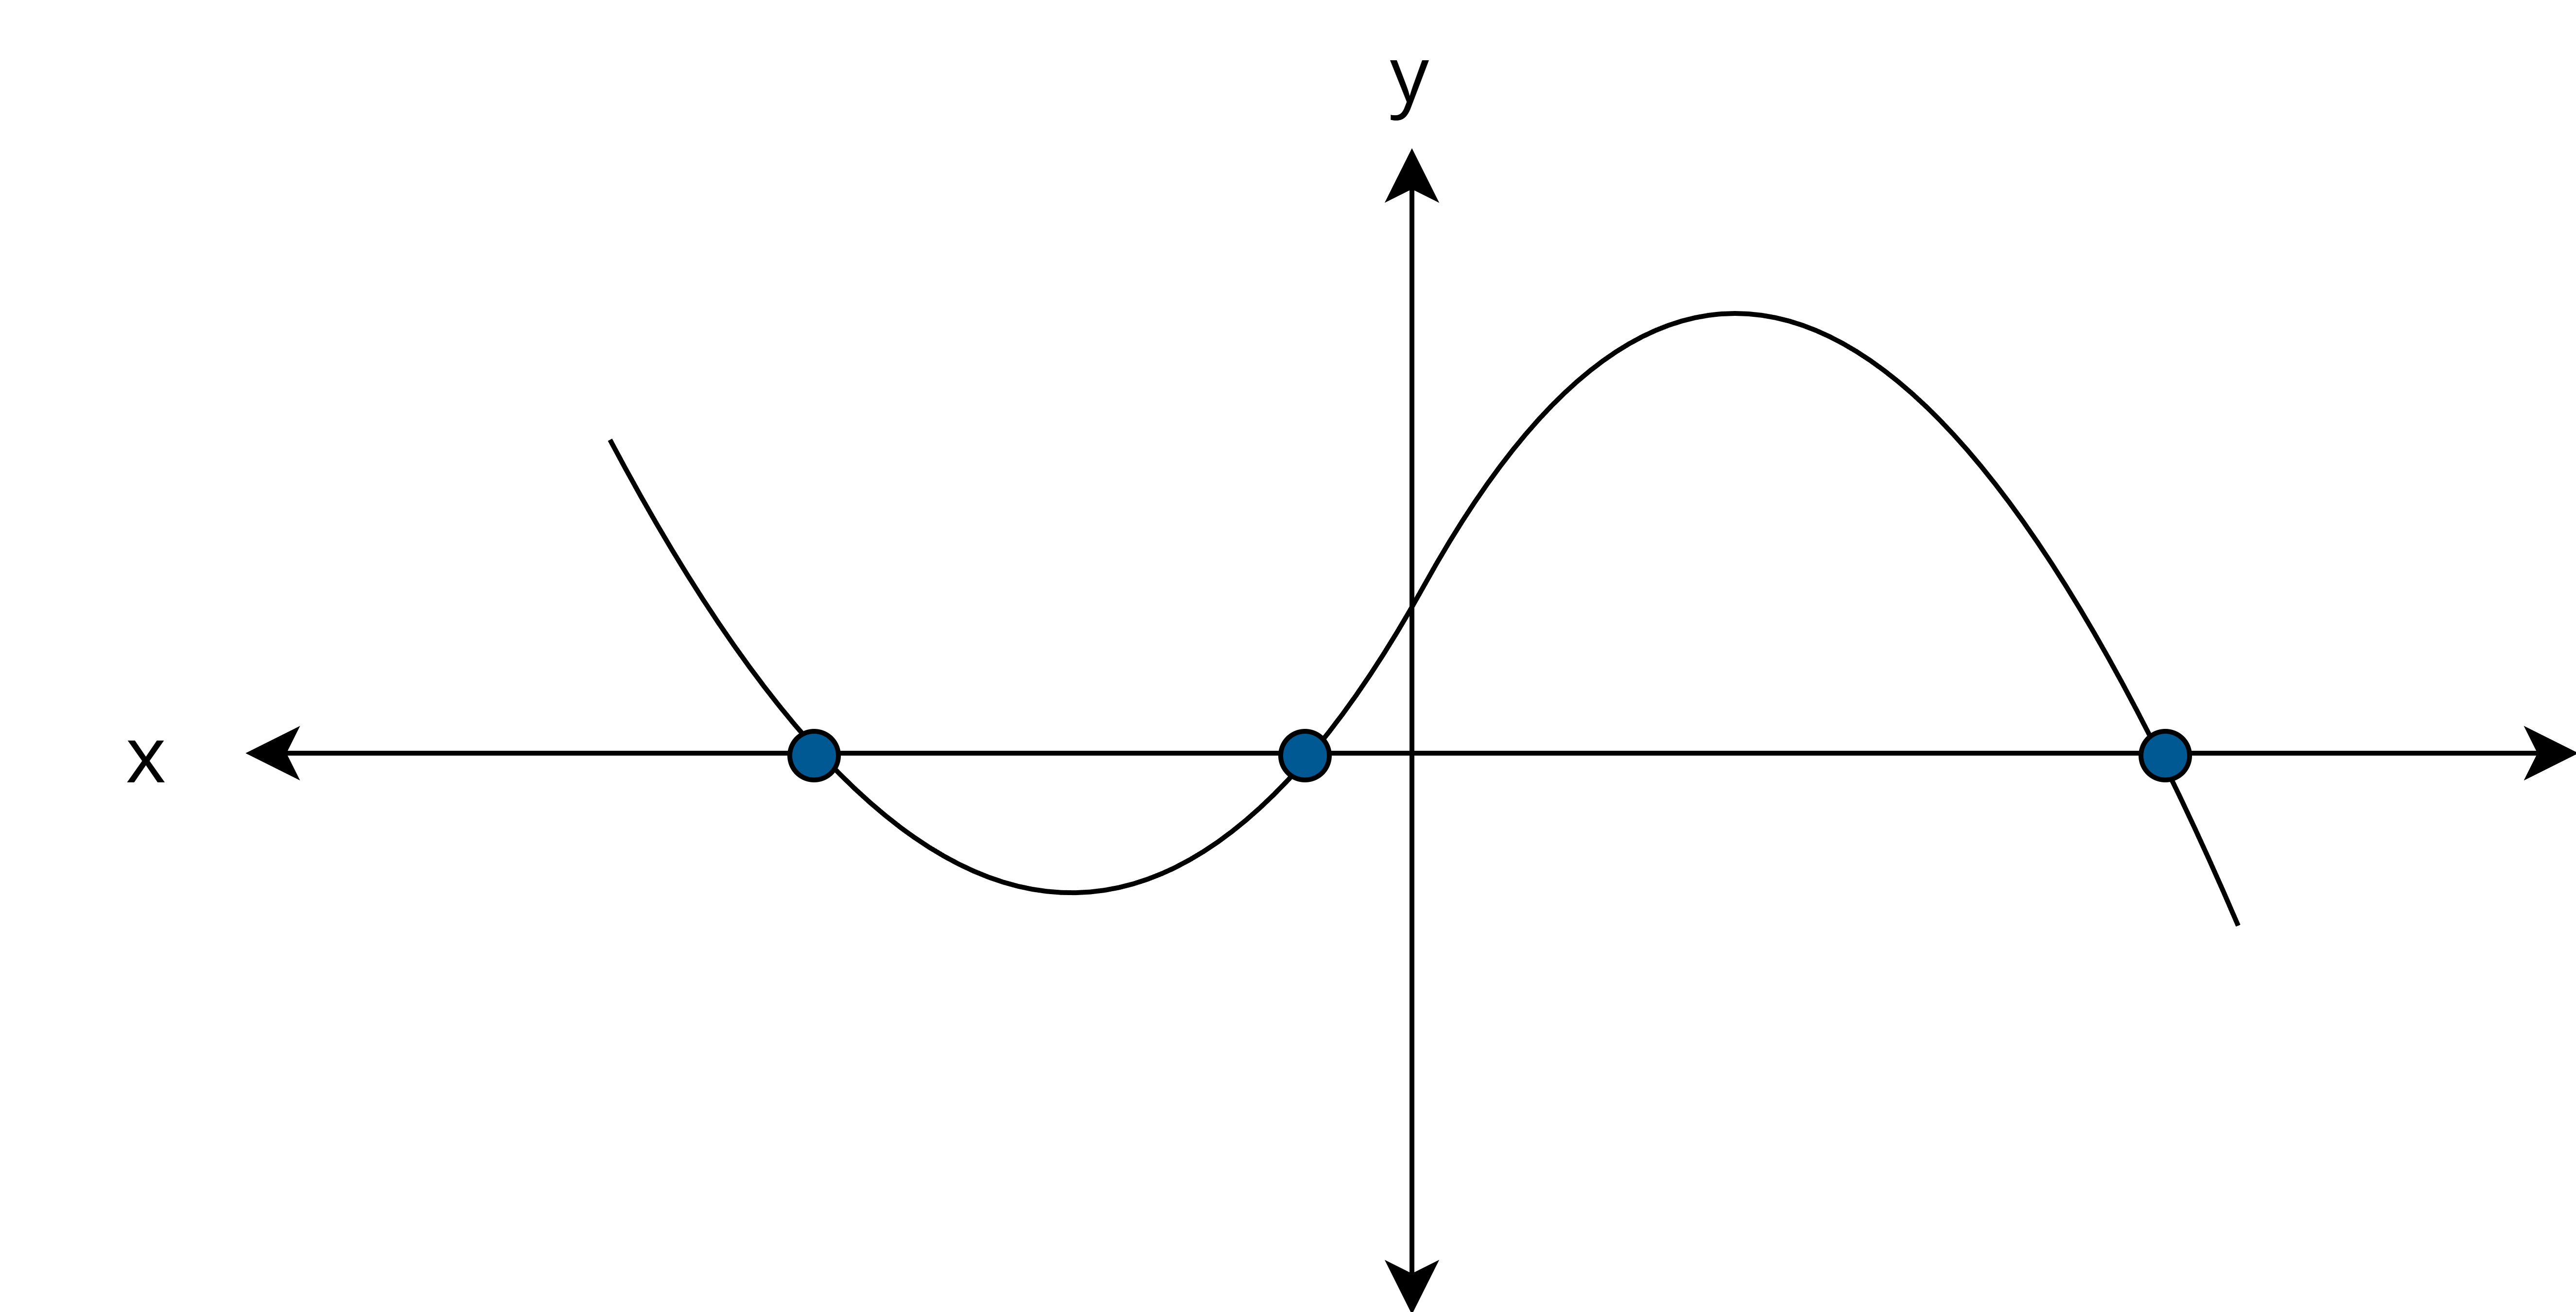
\includegraphics[width=\textwidth]{x_intercept_sequence18.png}
        \captionof{figure}{A graph showing the roots of a polynomial}
        \label{fig:x_intercept_sequence18}
    \end{center}

\item the \index{level spots}level spots on the graph (often the top of a hump or the bottom of a dip). Recall the derivative from the classes chapter: a polynomial whose value is the slope of the graph. The level spots are where the slope is zero, so you find the roots of the derivative.

    \begin{center}
        
\includegraphics[width=\textwidth]{extrema_sequence18.png}
        \captionof{figure}{A graph showing “level spots” of a polynomial.}
        \label{fig:extrema_sequence18}
    \end{center}
\end{itemize}

\index{polynomial!graphing}

For example, if you wanted to graph the polynomial $f(x) = -x^3 -x^2 +
6x$, you might plug in a few values that are easy to compute:

\begin{itemize}
\item $f(-2) = -8$
\item $f(-1) = -6$
\item $f(0) = 0$
\item $f(1) = 4$
\item $f(2) = 0$ 
\end{itemize}

So, right away, we know two roots: $x = 0$ and $x = 2$. Are there
others? We will not know until we factor the polynomial:
\begin{multline*}
  -x^3 -x^2 + 6x \\
  = (-1x)(x^2 + x - 6) \\
  = (-1x)(x + 3)(x - 2)
\end{multline*}
So, yes, there is a third root: $x = -3$

What about the level spots? Using the rule from the classes chapter (each
$cx^n$ becomes $ncx^{n-1}$), the derivative is $f'(x) = -3x^2 - 2x + 6$.
Where is that zero? Divide by $-3$:
\begin{multline*}
  -3x^2 -2x + 6 = 0 \\
  x^2 + \frac{2}{3}x - 2 = 0
\end{multline*}
We have a \index{quadratic formula}formula for quadratics like this:
\begin{multline*}
  x = -\frac{b}{2} \pm \frac{\sqrt{b^2 - 4c}}{2} \\
  = -\frac{\frac{2}{3}}{2} \pm \frac{\sqrt{\left(\frac{2}{3}\right)^2 - 4(-2)}}{2} \\
  = -\frac{1}{3} \pm \frac{\sqrt{\frac{4}{9} + 8}}{2} \\
  = -\frac{1}{3} \pm \frac{\sqrt{\frac{85}{9}}}{2} \\
  = -\frac{1}{3} \pm \frac{\sqrt{85}}{6} \\
  \approx 1.20 \text{ and } -1.87 
\end{multline*}

Now, you might plug those numbers in:
\begin{itemize}
\item $f(1.2) \approx 4.0 $
\item $f(-1.87) \approx -8.2$
\end{itemize}

\subsection{Leading term in graphing}\index{end behavior}

There is one more trick you need before you can draw a good graph of a
polynomial. As you go farther and farther to the left and right, where
does the function go? In other words, does the graph go up on both ends
(like a smile)? Or does it go down on both ends (like a frown)? Or
does the negative end go down (frowny) while the positive end go up
(smiley)? Or does the negative go up (smiley) and the positive end go
down (frowny)?

Assuming the polynomial is not constant, there are only those four
possibilities. It is determined entirely by the leading term of the
polynomial.  If the degree of the leading term is even, both ends go
in the same direction (both are smiley or both are frowny).  If the
coefficient of the leading term is positive, the right end goes up.
(Far from zero, the leading term is so much bigger than all the others
that it decides everything.)

\textbf{Worked example.} Describe the graph of $p(x) = x^3 - x$.

\textbf{Solution.} It factors as $x(x - 1)(x + 1)$, so it crosses the
$x$-axis at $-1$, 0, and 1, and the $y$-intercept is 0. The leading term
$x^3$ has odd degree and positive coefficient, so the graph comes up from
the bottom left and rises to the top right.

The graph we are working on has a leading term of $-1x^3$. The degree is odd, thus the ends go in different directions. The coefficient is negative, so the positive end points down.  Now, you can draw the graph, which should look something like this:
\begin{figure}[H]
    \centering
    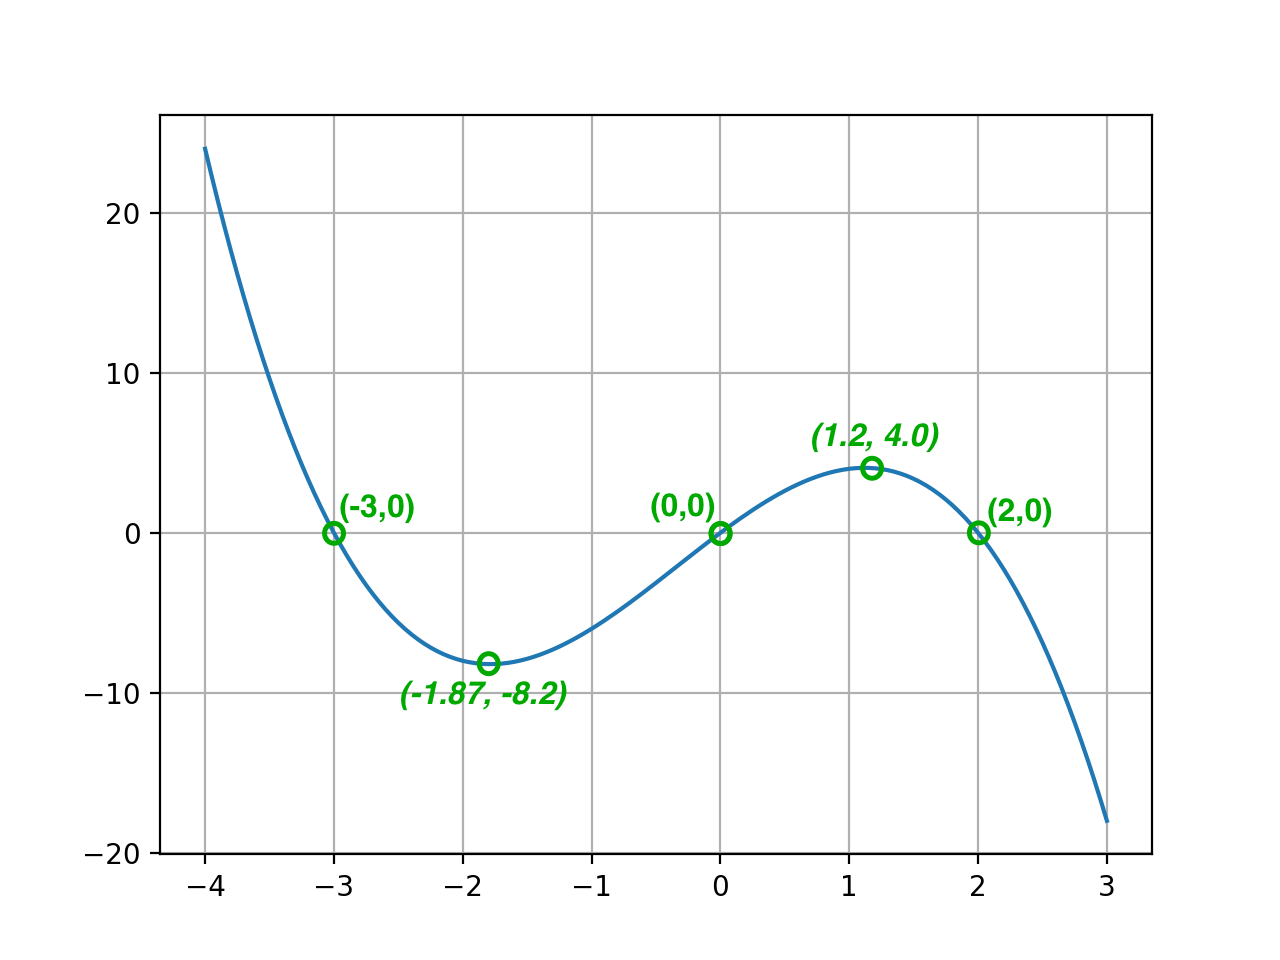
\includegraphics[width=\textwidth]{annotated_graph.png}
    \caption{A graph with roots and significant points.}
    \label{fig:annotated_graph}
\end{figure}


\section{Interpolating with Polynomials}
Let us say someone on a distant planet records video of a hammer being
thrown up into the air.  They send you three random frames of the
hammer in flight. Each frame has a timestamp, and you can clearly see
how high the hammer is in each one. Can you create a 2nd degree
polynomial that explains the entire flight of the hammer?

In other words, you have three points $(t_0, h_0), (t_1, h_1), (t_2, h_2)$.
\index{interpolation}Can you find $a,b,c$ such that the graph of $h = at^2 + bt + c$ passes
through all three points?

The answer is yes. In fact, \index{polynomial!through given points}given
any $n$ points with different $t$ values, there is exactly one polynomial
of degree at most $n-1$ that passes through all of them. (Two points
determine a line, which has degree 1. Three points determine a parabola,
degree 2.) Finding it is called \newterm{interpolation}.

There are a lot of variables floating around. Let us make it concrete:
The photos are taken at $t = 2$ seconds, $t = 3$ seconds, and $t = 4$
seconds. In those photos, the height of the hammer is $5m$, $7m$, and
$6m$. So, we want our polynomial to pass through these points: (2, 5),
(3, 7), (4,6).
\begin{figure}[H]
    \centering
    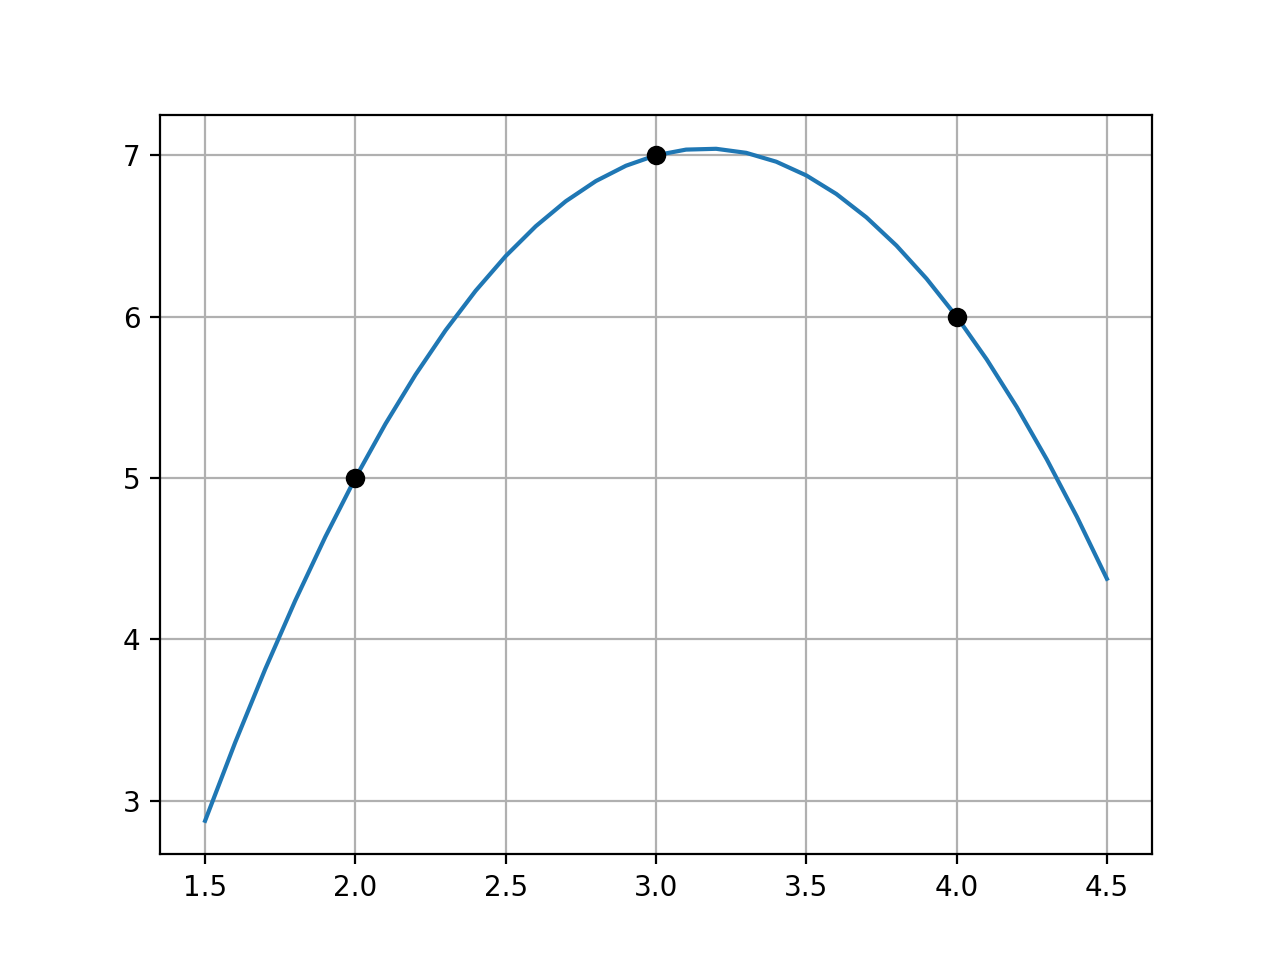
\includegraphics[width=0.45\textwidth]{interpolation.png} 
    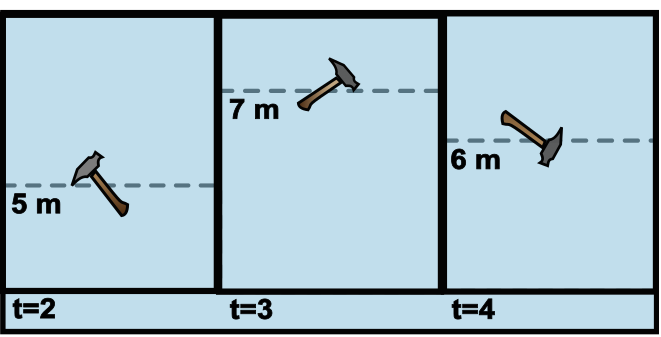
\includegraphics[width=0.45\textwidth]{hammer_1.png}
    \caption{Left: the graph of the hammer going through the given points. Right: the three hammer frames.}
    \label{fig:hammer_interpolation}
\end{figure}


How can you find that polynomial? Let us do it in small steps. Can you
create a 2nd degree polynomial that is not zero at $t = 2$, but is zero
at $t = 3$ and $t = 4$? Yes, you can: $(x - 3)(x - 4)$ has
exactly two roots at $t = 3$ and $t = 4$.  The value of this polynomial at
$t = 2$ is $(2 - 3)(2 - 4) = 2$. We really want it to be $5m$, so
we can divide the whole polynomial by 2 and multiply it by 5.

Now we have the polynomial:
\begin{equation*}
f_0(x) = \frac{5}{(2 - 3)(2 - 4)}(x - 3)(x - 4) = \frac{5}{2}x^2 - \frac{35}{2}x + 30
\end{equation*}
This is a second degree polynomial that is 5 at $t=2$ and 0 at $t=3$ and $t=4$.

Now, we create a polynomial that is 7 at $t=3$ and 0 at $t= 2$ and $t=4$:
\begin{equation*}
f_1(x) = \frac{7}{(3 - 2)(3 - 4)}(x - 2)(x - 4) = -7x^2 +42x - 56
\end{equation*}

Finally, we create a polynomial that is 6 at $t=4$ and zero at $t=2$ and $t=3$:
\begin{equation*}
f_2(x) = \frac{6}{(4 - 2)(4 - 3)}(x - 2)(x - 3) = 3x^2 - 15x + 18
\end{equation*}

Adding these three polynomials together gives you a new polynomial that touches all three points:
\begin{equation*}
  f(x) = \frac{5}{2}x^2 - \frac{35}{2}x + 30  - 7x^2 + 42x - 56 + 3x^2 - 15x + 18  = -\frac{3}{2}x^2 + \frac{19}{2}x -8
\end{equation*}

You can test this in Python with your \pytype{Polynomial} class. Create a file called \filename{test\_interpolation.py}. Add this code:
\begin{minted}{python}
from Polynomial import Polynomial
import matplotlib.pyplot as plt

in_x = [2,3,4]
in_y = [5,7,6]

pn = Polynomial([-8, 19/2, -3/2])
print(pn)

# These lists will hold our x and y values
x_list = []
y_list = []

# Starting x
current_x = 1.5

while current_x <= 4.5:
    # Evaluate pn at current_x
    current_y = pn(current_x)

    # Add x and y to respective lists
    x_list.append(current_x)
    y_list.append(current_y)

    # Move x forward
    current_x += 0.05
    
# Plot the curve
plt.plot(x_list, y_list)

# Plot black circles on the given points
plt.plot(in_x, in_y, "ko")
plt.grid(True)
plt.show()
\end{minted}

You should get a nice plot that shows the graph of the polynomial
passing through those three points.

In general, then, if you provide any three points $(t_0, h_0), (t_1, h_1), (t_2, h_2)$, there is a second degree polynomial that pass through all three:
\begin{equation*}
\frac{h_0}{(t_0 - t_1)(t_0 - t_2)}(x - t_1)(x - t_2) + \frac{h_1}{(t_1 - t_0)(t_1 - t_2)}(x - t_0)(x - t_2) + \frac{h_2}{(t_2 - t_0)(t_2 - t_1)}(x - t_0)(x - t_1)
\end{equation*}

What if you are given 9 points ($(t_0, h_0), (t_1, h_1), \ldots, (t_8,
h_8)$) and want to find a 8th degree polynomial that passes through
all of them? Just what you would expect:
\begin{equation*}
\frac{h_0}{(t_0 - t_1)(t_0 - t_2)\ldots(t_0 - t_8)}(x - t_1)(x - t_2)\ldots(x - t_8) + \ldots + \frac{h_8}{(t_8 - t_0)\ldots(t_8-t_7)}(x - t_0)\dots(x - t_7)
\end{equation*}

Mathematicians write this compactly with two symbols. You met $\Sigma$
(capital sigma) in the data chapters: it means ``add up.'' Its cousin
$\Pi$ (capital pi) means ``multiply together.'' \index{interpolation!general formula}Given $n$ points
$(t_0, h_0), \ldots, (t_{n-1}, h_{n-1})$, the polynomial of degree at
most $n-1$ that goes through them is
\begin{equation*}
  y =\sum_{i=0}^{n-1}\left ( \prod_{\stackrel{\!0\leq j\leq n-1}{j\neq i}}\frac{x-t_j}{t_i-t_j}\right ) h_i
\end{equation*}
Read it from the inside out: for each point $i$, multiply together the
factors $\frac{x - t_j}{t_i - t_j}$ for every other point $j$ (this is 1
at $t_i$ and 0 at every other $t_j$), scale by $h_i$, and add up the
results.

That would be tedious for a person to compute, but computers are perfect for this
stuff. Let us create a \index{from\_points method}method that creates instances of Polynomial
using interpolation.\footnote{Note that other textbooks or resources may refer to this as \textit{Lagrange Polynomial Interpolation}.}\index{Lagrange interpolation}

\subsection{Interpolating polynomials in python}\index{interpolation!in Python}

Your method will take two lists of numbers: one contains x-values and
the other contains y-values. So comment out the line that creates the
polynomial in \filename{test\_interpolation.py} and create it from two lists:
\begin{minted}{python}
in_x = [2,3,4]
in_y = [5,7,6]
# pn = Polynomial([-8, 19/2, -3/2])
pn = Polynomial.from_points(in_x, in_y)
print(pn)
\end{minted}

Add the following method to your Polynomial class in \filename{Polynomial.py}
\begin{minted}{python}
    @classmethod
    def from_points(cls, x_values, y_values):
        coef_count = len(x_values)

        # Sums start with a zero polynomial
        sum_pn = Polynomial([0.0] * coef_count)
        for i in range(coef_count):

            # Products start with the constant 1 polynomial
            product_pn = Polynomial([1.0])
            for j in range(coef_count):

                # Must skip j=i
                if j != i:
                    # (1x - x_values[j]) has a root at x_values[j]
                    factor_pn = Polynomial([-1 * x_values[j], 1])
                    product_pn = product_pn * factor_pn
                    
            # Scale so product_pn(x_values[i]) = y_values[i]
            scale_factor  = y_values[i] / product_pn(x_values[i])
            scaled_pn = scale_factor * product_pn

            # Add it to the sum
            sum_pn = sum_pn + scaled_pn
            
        return sum_pn  
\end{minted}

It should work exactly the same as before. You should get the same
polynomial printed out, $-1.50x^2 + 9.50x + -8.00$, and the same plot of
the curve passing through the three points.

The line \texttt{@classmethod} makes \pyfunction{from\_points} a method
of the class itself rather than of one polynomial, so you call it as
\texttt{Polynomial.from\_points(...)} to build a brand-new polynomial.

How about six points? Change \pyvar{in\_x} and \pyvar{in\_y} at the
start of \filename{test\_interpolation.py}:
\begin{minted}{python}
in_x = [1.7, 2, 2.7, 3.5, 4, 4.4]
in_y = [8, 12, 1, 4, -1, 6]
\end{minted}

You should get a degree 5 polynomial that passes through all six points:
\begin{equation*}
11.21x^5 - 171.05x^4 + 1019.44x^3 - 2957.53x^2 + 4161.78x - 2258.75  
\end{equation*}
It should look like this:

\begin{figure}[H]
    \centering
    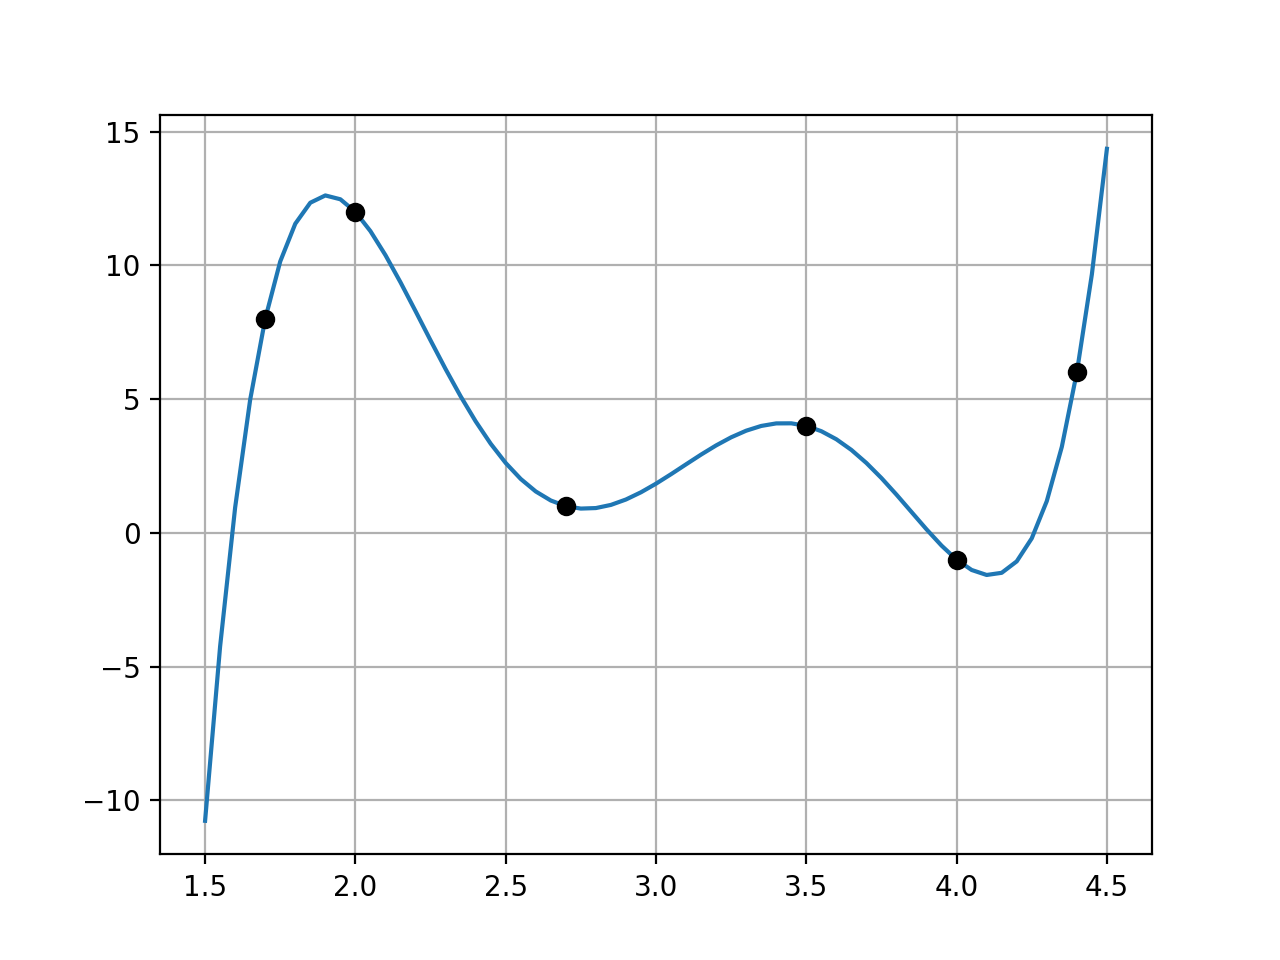
\includegraphics[width=0.7\textwidth]{fiveinterp.png}
    \caption{Interpolating six points with a degree 5 polynomial.}
    \label{fig:fiveinterp}
\end{figure}

\begin{Exercise}[title={Interpolate by hand}, label=poly3_2]
Find the parabola through $(0, 1)$, $(1, 0)$, and $(2, 3)$ using the
three-polynomial method from this chapter. Check your answer at all three
points.
\end{Exercise}
\begin{Answer}[ref=poly3_2]
$f_0 = \frac{1}{(0-1)(0-2)}(x-1)(x-2) = \frac{1}{2}(x^2 - 3x + 2)$.
$f_1 = \frac{0}{\ldots}(\ldots) = 0$.
$f_2 = \frac{3}{(2-0)(2-1)}x(x-1) = \frac{3}{2}(x^2 - x)$.
Adding: $p(x) = 2x^2 - 3x + 1$. Check: $p(0) = 1$, $p(1) = 0$,
$p(2) = 8 - 6 + 1 = 3$.
\end{Answer}

\begin{Exercise}[title={Interpolating a Line}, label=poly3_1]
Find the polynomial of degree at most $1$ through the points $(0, 1)$ and $(2, 5)$.
\end{Exercise}
\begin{Answer}[ref=poly3_1]
The slope is $\frac{5-1}{2-0} = 2$ and the intercept is $1$, so $p(x) = 2x + 1$.
\end{Answer}
